\documentclass{article}

% Set geometry
\usepackage[a4paper]{geometry}
\setlength\parindent{0pt}

% Show header and footer
\usepackage{fancyhdr}
\pagestyle{fancy}
\fancyhf{}
\lhead{Database System Implementation Practical 3}
\rhead{Candidate Number: 589087}
\cfoot{\thepage}

% Show figures
\usepackage{graphicx}

% Show code
\usepackage{listings}
\usepackage{color}

\definecolor{dkgreen}{rgb}{0,0.6,0}
\definecolor{gray}{rgb}{0.5,0.5,0.5}
\definecolor{mauve}{rgb}{0.58,0,0.82}

\lstset{frame=tb,
  language=C++,
  aboveskip=3mm,
  belowskip=3mm,
  showstringspaces=false,
  columns=flexible,
  basicstyle={\small\ttfamily},
  numbers=none,
  numberstyle=\tiny\color{gray},
  keywordstyle=\color{blue},
  commentstyle=\color{dkgreen},
  stringstyle=\color{mauve},
  breaklines=true,
  breakatwhitespace=true,
  tabsize=3
}

\begin{document}
\begin{titlepage}
{\centering
{\LARGE\bfseries Database System Implementation Practical 3}

\vspace{0.5cm}

{\Large Join Algorithms}

\vspace{2cm}

{\large Candidate Number: 589087}

\vspace{0.1cm}

{\large 08 March, 2015}

}

\vfill

\end{titlepage}
\newpage
\newpage
\section{Performance Test 1 - Original Configuration}

We used the original configuration in the first test, that is 50 buffer pages, 10k records in R and 2.5k records in S. The raw output of the algorithms are shown below.
\begin{center}
\begin{verbatim}
>>----------Test 1: Origional settings----------
Settings      # Buf Pages     # Rec in R     # Rec in S
                       50          10000           2500
Results         Avg # Pin   Avg # Misses   Avg Duration
Tuple Join         596469         511315       1.580910
Block Join          66787           1082       0.250078
Index Join             16              6       0.000044

>>----------End of Test 1: Origional settings----------
\end{verbatim}
\end{center}
We illustrate the results by two bar charts. The running time and pin misses of tuple join algorithm are the highest, while block nested loop join has significantly less misses and time, and index nested loop join's pin misses and duration are almost negligible.


\begin{figure}[!htbp]
  \centering
  \makebox[\textwidth][c]{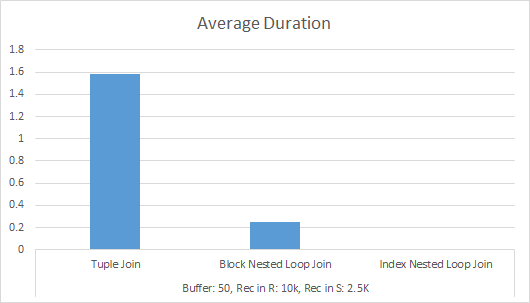
\includegraphics[width=0.6\textwidth]{11}}
  \caption{Average pin requests and pin misses}
    \label{fig: 1-1}
\end{figure}
\begin{figure}[!htbp]
  \centering
  \makebox[\textwidth][c]{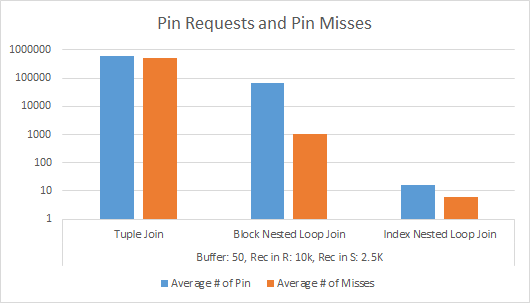
\includegraphics[width=0.6\textwidth]{12}}
  \caption{Average duration}
    \label{fig: 1-2}
\end{figure}

\newpage
\section{Performance Test 2 - Variable Buffer Size}
In the second test, we set the relation size R to 10k and S to 2.5k and vary the buffer size from $2^4$, $2^6$, $2^8$ to $2^{10}$. The raw data is shown below and the bar charts are given in the next page. \\

For the a-tuple-at-a-time join, the pin misses are significantly affected by small buffer size. As illustrated in figure \ref{fig: 2-1} and \ref{fig: 2-2}, compared to 16 buffer pages, the pin misses using 64 buffer pages are decreased by three order of magnitude, and the duration is decreased by 26\%. However, given the current configuration of numbers of records in R and S, larger buffer pages ($>$64) have less impact on the number of pin misses and duration.\\

The buffer size has similar impact on the number of misses of block nested loop join. However, the performance of index nested loop join showed no apparent difference under different buffer size.
\begin{center}
\begin{verbatim}
>>----------Test 2: Variant buffer size----------
Settings      # Buf Pages     # Rec in R     # Rec in S
                       16          10000           2500
Results         Avg # Pin   Avg # Misses   Avg Duration
Tuple Join         596469         553215       1.602876
Block Join          68271           2590       0.253056
Index Join             16              6       0.000042

Settings      # Buf Pages     # Rec in R     # Rec in S
                       64          10000           2500
Results         Avg # Pin   Avg # Misses   Avg Duration
Tuple Join         596469            788       1.189948
Block Join          66734           1017       0.251087
Index Join             16              6       0.000045

Settings      # Buf Pages     # Rec in R     # Rec in S
                      256          10000           2500
Results         Avg # Pin   Avg # Misses   Avg Duration
Tuple Join         596469            747       1.245568
Block Join          66522            776       0.256826
Index Join             16              6       0.000050

Settings      # Buf Pages     # Rec in R     # Rec in S
                     1024          10000           2500
Results         Avg # Pin   Avg # Misses   Avg Duration
Tuple Join         596469            459       1.268922
Block Join          66522            459       0.259093
Index Join             16              2       0.000044

>>----------End of Test 2: Variant buffer size----------
\end{verbatim}
\end{center}


\newpage
\begin{figure}[!htbp]
  \centering
  \makebox[\textwidth][c]{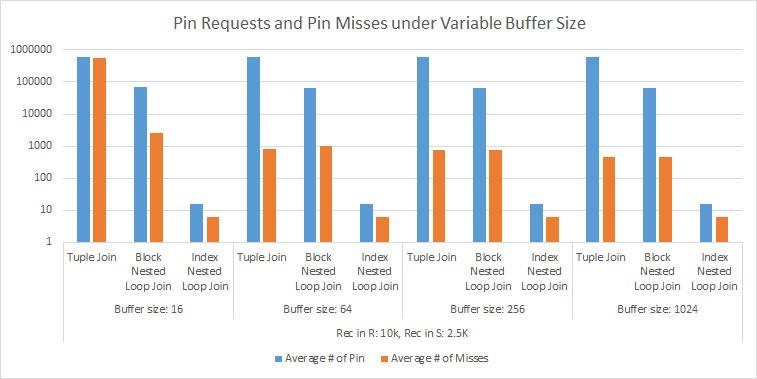
\includegraphics[width=1.0\textwidth]{21}}
  \caption{Average pin requests and pin misses under variable buffer size}
    \label{fig: 2-1}
\end{figure}
\begin{figure}[!htbp]
  \centering
  \makebox[\textwidth][c]{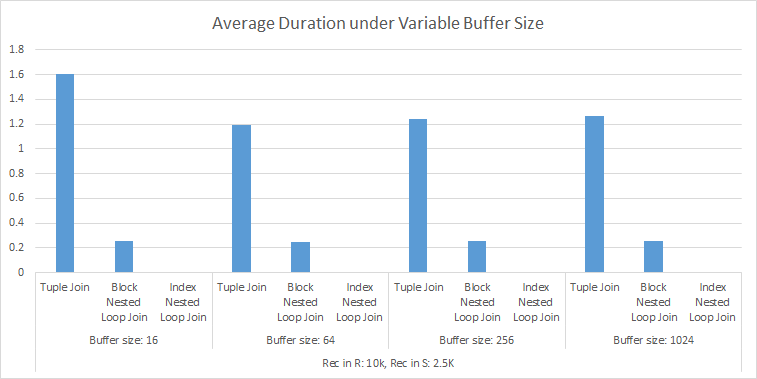
\includegraphics[width=1.0\textwidth]{22}}
  \caption{Average duration under variable buffer size}
    \label{fig: 2-2}
\end{figure}

\newpage
\section{Performance Test 3 - Variable R Size}
In the third test, we set the buffer size to 50, relation size of S to 2.5k and the relation size of R to $2^i$, where i is in the set of \{1, 3, ..., 13\}. The raw output and graphs are shown below. \\


As illustrated in figure \ref{fig: 3-2} and \ref{fig: 3-3}, 1) the pin misses and duration of tuple join grows very fast as the relation size R increases (NB. the scales of axes in the graphs are different); 2) block nested loop join has a stable pin misses and duration when the size of R is smaller or equal to 512, but then they grows dramatically when the R is greater than 512; 3) the index nested loop join seems has not influenced by the size of relation R.
\begin{verbatim}
>>----------Test 3: Variant R size----------
Settings      # Buf Pages     # Rec in R     # Rec in S
                       50              2           2500
Results         Avg # Pin   Avg # Misses   Avg Duration
Tuple Join            127            109       0.000518
Block Join             74             52       0.000210
Index Join             16              4       0.000017

Settings      # Buf Pages     # Rec in R     # Rec in S
                       50              8           2500
Results         Avg # Pin   Avg # Misses   Avg Duration
Tuple Join            457            413       0.001442
Block Join             86             52       0.000325
Index Join             16              4       0.000018

Settings      # Buf Pages     # Rec in R     # Rec in S
                       50             32           2500
Results         Avg # Pin   Avg # Misses   Avg Duration
Tuple Join           1786           1613       0.005064
Block Join            143             54       0.000853
Index Join             16              4       0.000017

Settings      # Buf Pages     # Rec in R     # Rec in S
                       50            128           2500
Results         Avg # Pin   Avg # Misses   Avg Duration
Tuple Join           7105           6446       0.019767
Block Join            374             61       0.002769
Index Join             16              3       0.000017

Settings      # Buf Pages     # Rec in R     # Rec in S
                       50            512           2500
Results         Avg # Pin   Avg # Misses   Avg Duration
Tuple Join          28398          25629       0.078892
Block Join           1315             92       0.010374
Index Join             16              6       0.000025

Settings      # Buf Pages     # Rec in R     # Rec in S
                       50           2048           2500
Results         Avg # Pin   Avg # Misses   Avg Duration
Tuple Join         113552         102390       0.314852
Block Join           5114            259       0.043508
Index Join             16              6       0.000040

Settings      # Buf Pages     # Rec in R     # Rec in S
                       50           8192           2500
Results         Avg # Pin   Avg # Misses   Avg Duration
Tuple Join         481564         416531       1.314850
Block Join          47653            886       0.200664
Index Join             16              6       0.000039

>>----------End of Test 3: Variant R size----------
\end{verbatim}

\newpage
\begin{figure}[!htbp]
  \centering
  \makebox[\textwidth][c]{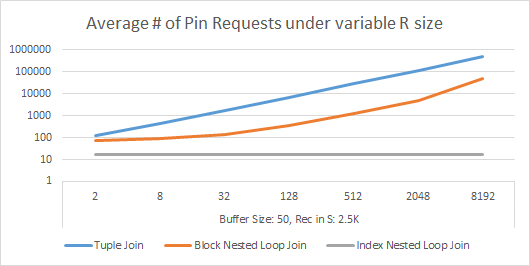
\includegraphics[width=0.7\textwidth]{31}}
  \caption{Average pin requests under variable R size}
    \label{fig: 3-1}
\end{figure}
\begin{figure}[!htbp]
  \centering
  \makebox[\textwidth][c]{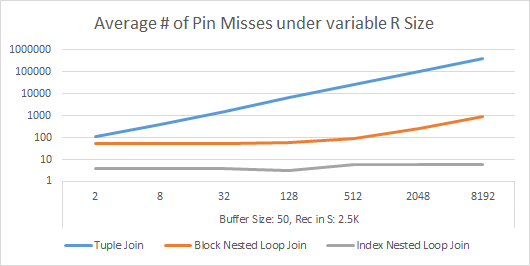
\includegraphics[width=0.7\textwidth]{32}}
  \caption{Average pin misses under variable R size}
    \label{fig: 3-2}
\end{figure}
\begin{figure}[!htbp]
  \centering
  \makebox[\textwidth][c]{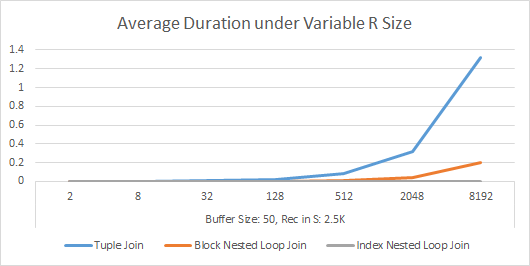
\includegraphics[width=0.7\textwidth]{33}}
  \caption{Average duration under variable R size}
    \label{fig: 3-3}
\end{figure}

\newpage
\section{Performance Test 4 - Variable S Size}
In the fourth test, we set the buffer size to 50, relation size R to 10k and the relation size S to $2^i$, where i is in the set of \{1, 3, ..., 13\}. The raw output and graphs are shown below. \\


If the relation S is smaller than or equal to 512, then the pin misses and duration is stable for all the three algorithms, nevertheless the pin misses of tuple join and block nested loop join are 3 order of magnitude larger than index nested loop join. If the relation S is grater 512, the pin misses of index nested loop join and block nested loop join grow gradually, while tuple join's pin misses grow very fast. We can see a similar trend on duration change. 

\begin{verbatim}
>>----------Test 3: Variant S size----------
Settings      # Buf Pages     # Rec in R     # Rec in S
                       50          10000              2
Results         Avg # Pin   Avg # Misses   Avg Duration
Tuple Join          86469            747       0.064967
Block Join          66481            762       0.057190
Index Join             16              5       0.000036

Settings      # Buf Pages     # Rec in R     # Rec in S
                       50          10000              8
Results         Avg # Pin   Avg # Misses   Avg Duration
Tuple Join          86469            747       0.067563
Block Join          66481            754       0.057883
Index Join             16              5       0.000036

Settings      # Buf Pages     # Rec in R     # Rec in S
                       50          10000             32
Results         Avg # Pin   Avg # Misses   Avg Duration
Tuple Join          86469            747       0.076883
Block Join          66481            754       0.059735
Index Join             16              5       0.000031

Settings      # Buf Pages     # Rec in R     # Rec in S
                       50          10000            128
Results         Avg # Pin   Avg # Misses   Avg Duration
Tuple Join         106469            747       0.118565
Block Join          66493            781       0.067305
Index Join             16              5       0.000036

Settings      # Buf Pages     # Rec in R     # Rec in S
                       50          10000            512
Results         Avg # Pin   Avg # Misses   Avg Duration
Tuple Join         186469            747       0.287018
Block Join          66541            824       0.096548
Index Join             16              5       0.000041

Settings      # Buf Pages     # Rec in R     # Rec in S
                       50          10000           2048
Results         Avg # Pin   Avg # Misses   Avg Duration
Tuple Join         496469           2336       0.954325
Block Join          66727           1014       0.214366
Index Join             16              6       0.000041

Settings      # Buf Pages     # Rec in R     # Rec in S
                       50          10000           8192
Results         Avg # Pin   Avg # Misses   Avg Duration
Tuple Join        1766469        1722204       5.059543
Block Join          67489           1783       0.751575
Index Join             16              7       0.000054

>>----------End of Test 3: Variant S size----------
\end{verbatim}
\newpage
\begin{figure}[!htbp]
  \centering
  \makebox[\textwidth][c]{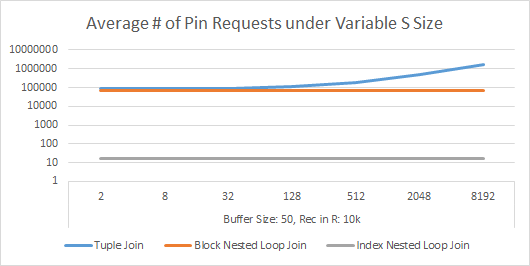
\includegraphics[width=0.7\textwidth]{41}}
  \caption{Average pin requests under variable S size}
    \label{fig: 4-1}
\end{figure}
\begin{figure}[!htbp]
  \centering
  \makebox[\textwidth][c]{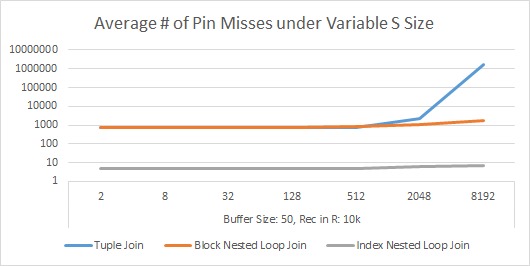
\includegraphics[width=0.7\textwidth]{42}}
  \caption{Average pin misses under variable S size}
    \label{fig: 4-2}
\end{figure}
\begin{figure}[!htbp]
  \centering
  \makebox[\textwidth][c]{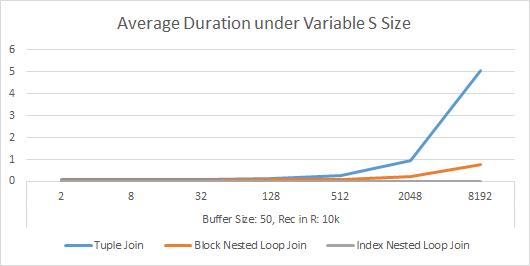
\includegraphics[width=0.7\textwidth]{43}}
  \caption{Average duration under variable S size}
    \label{fig: 4-3}
\end{figure}


\newpage
\section{Code - tuplejoin.cpp}
\begin{lstlisting}
#include <stdio.h>
#include <stdlib.h>
#include <string.h>
#include <time.h>

#include "../include/minirel.h"
#include "../include/heapfile.h"
#include "../include/scan.h"
#include "../include/join.h"
#include "../include/relation.h"
#include "../include/bufmgr.h"
#include <ctime>

using namespace std;

//---------------------------------------------------------------
// Each join method takes in at least two parameters :
// - specOfS
// - specOfR
//
// They specify which relations we are going to join, which 
// attributes we are going to join on, the offsets of the 
// attributes etc.  specOfS specifies the inner relation while
// specOfR specifies the outer one.
//
//You can use MakeNewRecord() to create the new result record.
//
// Remember to clean up before exiting by "delete"ing any pointers
// that you "new"ed.  This includes any Scan/BTreeFileScan that 
// you have opened.
//---------------------------------------------------------------


void TupleNestedLoopJoin(JoinSpec specOfR, JoinSpec specOfS, 
	long& pinRequests, long& pinMisses, double& duration)
{

	// Reset stat of buffer manager
	MINIBASE_BM->ResetStat();

	// Create a timer
	clock_t start = clock();

	Status status = OK;
	
	// Initialise scan on relation R.
	Scan *scanOnR = specOfR.file->OpenScan(status);
	if (status != OK) cerr << "ERROR : cannot open scan on the heapfile R.\n";
	
	// Create new relation for joined result.
	HeapFile *joinedRelation = new HeapFile(NULL, status); 
	if (status != OK) cerr << "Cannot create new file for joined relation\n";

	// Initialise record ids and record pointers.
	RecordID ridR, ridS, ridJoined;
	char *recPtrR = new char[specOfR.recLen];
	char *recPtrS = new char[specOfS.recLen];
	char *recPtrRandS = new char[specOfR.recLen + specOfS.recLen];
	// GetNext takes length of record (3rd parameter), returns next rid and record
	// in a relation (heapfile). See join.cpp L68-71.
	while ( scanOnR->GetNext( ridR, recPtrR, specOfR.recLen) == OK) 
	{
		// Initialise scan on relation S.
		Scan *scanOnS = specOfS.file->OpenScan(status);
		if (status != OK) cerr << "ERROR : cannot open scan on the heapfile S.\n";
		
		while( scanOnS->GetNext( ridS, recPtrS, specOfS.recLen) == OK)
		{
			// recPtr{S, R} are defined as char*, recPtrS[specOfS.offset] 
			// gets the first byte of the join attribute, then get the address, 
			// and cast to int pointer.
			int* attrToJoinOnS = (int*)&recPtrS[specOfS.offset];
			int* attrToJoinOnR = (int*)&recPtrR[specOfR.offset];
			if( *attrToJoinOnR == *attrToJoinOnS)
			{
				// join two records and jopined record is in recPtrRandS
				MakeNewRecord( recPtrRandS, recPtrR, recPtrS, specOfR.recLen, specOfS.recLen);	
				joinedRelation -> InsertRecord( recPtrRandS, specOfR.recLen + specOfS.recLen, ridJoined);
			}
		}

		delete scanOnS;
	}

	// clean up
	delete scanOnR;
	delete[] recPtrR, recPtrS, recPtrRandS;

	delete joinedRelation;

	// get stat;
	MINIBASE_BM->GetStat(pinRequests, pinMisses);
	duration = ( clock() - start) / (double) CLOCKS_PER_SEC;
}
\end{lstlisting}

\newpage
\section{Code - blockjoin.cpp}
\begin{lstlisting}
#include <stdio.h>
#include <stdlib.h>
#include <string.h>
#include <time.h>

#include "../include/minirel.h"
#include "../include/heapfile.h"
#include "../include/scan.h"
#include "../include/join.h"
#include "../include/relation.h"
#include "../include/bufmgr.h"

//---------------------------------------------------------------
// Each join method takes in at least two parameters :
// - specOfS
// - specOfR
//
// They specify which relations we are going to join, which 
// attributes we are going to join on, the offsets of the 
// attributes etc.  specOfS specifies the inner relation while
// specOfR specifies the outer one.
//
//You can use MakeNewRecord() to create the new result record.
//
// Remember to clean up before exiting by "delete"ing any pointers
// that you "new"ed.  This includes any Scan/BTreeFileScan that 
// you have opened.
//---------------------------------------------------------------

void BlockNestedLoopJoin(JoinSpec specOfR, JoinSpec specOfS, 
	int blocksize, long& pinRequests, long& pinMisses, double& duration)
{
	// Reset stat of buffer manager
	MINIBASE_BM->ResetStat();

	// Create a timer
	clock_t start = clock();

	Status status = OK;

	// Initialise scan on relation R.
	Scan *scanOnR = specOfR.file->OpenScan(status);
	if (status != OK) cerr << "ERROR : cannot open scan on the heapfile R.\n";

	// Create new relation for joined result.
	HeapFile *joinedRelation = new HeapFile(NULL, status); 
	if (status != OK) cerr << "Cannot create new file for joined relation\n";
	
	// Initialise record ids and record pointers.
	RecordID ridR, ridS, ridJoined;
	char *recPtrR = new char[specOfR.recLen];
	char *recBlockPtrR = new char[blocksize];
	char *recPtrS = new char[specOfS.recLen];
	char *recPtrRandS = new char[specOfR.recLen + specOfS.recLen];

	bool done = false;

	// for each block b in R
	while(!done)
	{
		int numOfRecInBlockR = blocksize / specOfR.recLen;
		int numOfRecInRRead = 0;
		// Get the block
		for(int i = 0; i < numOfRecInBlockR; i++)
		{
			if( scanOnR->GetNext( ridR, recBlockPtrR + i*specOfR.recLen, specOfR.recLen) != OK)
			{
				// reach the end of relation R
				done = true;
				break;
			}
			numOfRecInRRead++;
		}

		// Initialise scan on relation R.
		Scan *scanOnS = specOfS.file->OpenScan(status);
		if (status != OK) cerr << "ERROR : cannot open scan on the heapfile S.\n";		

		// for each tuple in S
		while( scanOnS->GetNext( ridS, recPtrS, specOfS.recLen) == OK)
		{
			// for each tuple in r
			for(int i = 0; i < numOfRecInRRead; i++)
			{
				// extract record from record block
				memcpy(recPtrR, recBlockPtrR + i * specOfR.recLen, specOfR.recLen);

				// match r with s
				int* attrToJoinOnS = (int*)&recPtrS[specOfS.offset];
				int* attrToJoinOnR = (int*)&recPtrR[specOfR.offset];
				
				if( *attrToJoinOnR == *attrToJoinOnS)
				{
					// join two records and jopined record is in recPtrRandS
					MakeNewRecord( recPtrRandS, recPtrR, recPtrS, specOfR.recLen, specOfS.recLen);	
					joinedRelation -> InsertRecord( recPtrRandS, specOfR.recLen + specOfS.recLen, ridJoined);
				}
			}
		}

		delete scanOnS;
	}

	delete[] recPtrR, recPtrS, recBlockPtrR, recPtrS;
	delete joinedRelation;
	delete scanOnR;

	// get stat
	MINIBASE_BM->GetStat(pinRequests, pinMisses);
	duration = ( clock() - start) / (double) CLOCKS_PER_SEC;
}
\end{lstlisting}

\newpage
\section{Code - indexjoin.cpp}
\begin{lstlisting}
#include <stdio.h>
#include <stdlib.h>
#include <string.h>
#include <time.h>

#include "../include/minirel.h"
#include "../include/heapfile.h"
#include "../include/scan.h"
#include "../include/join.h"
#include "../include/btfile.h"
#include "../include/btfilescan.h"
#include "../include/relation.h"
#include "../include/bufmgr.h"



//---------------------------------------------------------------
// Each join method takes in at least two parameters :
// - specOfS
// - specOfR
//
// They specify which relations we are going to join, which 
// attributes we are going to join on, the offsets of the 
// attributes etc.  specOfS specifies the inner relation while
// specOfR specifies the outer one.
//
//You can use MakeNewRecord() to create the new result record.
//
// Remember to clean up before exiting by "delete"ing any pointers
// that you "new"ed.  This includes any Scan/BTreeFileScan that 
// you have opened.
//---------------------------------------------------------------


void IndexNestedLoopJoin(JoinSpec specOfR, JoinSpec specOfS, 
	long& pinRequests, long& pinMisses, double& duration)
{
	// Reset stat of buffer manager
	MINIBASE_BM->ResetStat();

	// Create a timer
	clock_t start = clock();

	Status status = OK;

	// Create new relation for joined result.
	HeapFile *joinedRelation = new HeapFile(NULL, status); 
	if (status != OK) cerr << "Cannot create new file for joined relation\n";

	/////////////////////////////////////////////////
	//Build B+ Tree for inner relation //////////////
	/////////////////////////////////////////////////
	Scan *scanOnS = specOfS.file->OpenScan(status);
	if (status != OK) cerr << "ERROR : cannot open scan on the heapfile S.\n";
	BTreeFile *btree = new BTreeFile( status, "BTreeS", ATTR_INT, sizeof(int));

	char *recS = new char[specOfS.recLen];
	RecordID ridS;
	// Insert records in S to b+ tree
	while( scanOnS->GetNext(ridS, recS, specOfS.recLen))
	{
		btree->Insert(recS + specOfS.offset, ridS);
	}

	// clean up
	delete scanOnS;
	delete[] recS;

	/////////////////////////////////////////////////
	//Join R to S////////////////////////////////////
	/////////////////////////////////////////////////

	RecordID ridR, ridJoined;
	char *recPtrR = new char[specOfR.recLen];
	char *recPtrS = new char[specOfS.recLen];
	char *recPtrRandS = new char[specOfR.recLen + specOfS.recLen];

	// Initialise scan on relation R.
	Scan *scanOnR = specOfR.file->OpenScan(status);
	if (status != OK) cerr << "ERROR : cannot open scan on the heapfile R.\n";

	// for each record in R
	while( scanOnR->GetNext(ridR, recPtrR, specOfR.recLen))
	{
		BTreeFileScan  *btreeScan = (BTreeFileScan *)btree->OpenScan(NULL, NULL);
		
		// for each entry in b+ tree
		int key;
		while( btreeScan->GetNext(ridS, &key) == OK)
		{
			// get record from relation S
			specOfS.file->GetRecord(ridS, recPtrS, specOfS.recLen);

			// match
			int* attrToJoinOnS = (int*)&recPtrS[specOfS.offset];
			int* attrToJoinOnR = (int*)&recPtrR[specOfR.offset];
			if( *attrToJoinOnR == *attrToJoinOnS)
			{
				// join two records and jopined record is in recPtrRandS
				MakeNewRecord( recPtrRandS, recPtrR, recPtrS, specOfR.recLen, specOfS.recLen);	
				joinedRelation -> InsertRecord( recPtrRandS, specOfR.recLen + specOfS.recLen, ridJoined);
			}	
		}

		delete btreeScan;
	}


	// clean up
	delete btree;
	delete scanOnR;
	delete[] recPtrS, recPtrR, recPtrRandS;
	delete joinedRelation;

	// get stat;
	MINIBASE_BM->GetStat(pinRequests, pinMisses);
	duration = ( clock() - start) / (double) CLOCKS_PER_SEC;
}
\end{lstlisting}

\newpage
\section{Code - main.cpp}
\begin{lstlisting}
#include <stdlib.h>
#include <time.h>
#include <ctype.h>

#include "include/minirel.h"
#include "include/bufmgr.h"
#include "include/heapfile.h"
#include "include/join.h"
#include "include/relation.h"

#include <sys/select.h>
#include <sys/time.h>
#include <unistd.h>
#include <iomanip>
#include <stdio.h>
#include <cstdio>

int MINIBASE_RESTART_FLAG = 0;// used in minibase part

#define NUM_OF_DB_PAGES  2000 // define # of DB pages
#define NUM_OF_BUF_PAGES_ORIGINAL 50 // origional settings 
#define NUM_OF_REC_IN_R_ORIGINAL 10000 // origional settings 
#define NUM_OF_REC_IN_S_ORIGINAL 2500 // origional settings 

#define NUM_OF_BUF_MAX_PAGES 1024 // for the experiment on different buffer size
#define NUM_OF_MAX_REC_R 10000 // for the experiment on different R size 
#define NUM_OF_MAX_REC_S 10000 // for the experiment on different S size
#define NUM_OF_REPETITION_TASK1 10
#define NUM_OF_REPETITION_TASK2 5
#define NUM_OF_REPETITION_TASK3 2

using namespace std;

void perfCompTask1();
void perfCompTask2();
void perfCompTask3(bool isVarR);

void callJoins( int numOfBuf, int numOfRecR, int numOfRecS, 
	long pinNo[3], long pinMisses[3], double duration[3] );

void printTestTitle(int testNo, bool isStart, const char* nameOfTest);
void printSettings(int buf, int recR, int recS);
void printResults(double avgPinNo[3], double avgPinMisses[3], double avgDuration[3]);

static inline void loadbar(unsigned int x, unsigned int n, unsigned int w = 40);

int main()
{
	remove( "data.txt" ); 
	perfCompTask1(); // orgional settings
	perfCompTask2(); // variable buffer size
	perfCompTask3(true); // variable R
	perfCompTask3(false); // variable S
	printf("%s\n\n", ">> All done! See data.txt for output.");
	return 1;
}


//--------------------------------------------------
// Performance comparison 1
// Using origional settings, repeat NUM_OF_REPETITION_TASK1 times, 
// calculate average pin number, pin misses and duration
//-------------------------------------------------- 
void perfCompTask1()
{
	int count = 0;
	double *avgPinNo = new double[3];
	double *avgPinMisses = new double[3];
	double *avgDuration = new double[3];

	//printf("%s\n", ">>----------Test 1: Origional settings----------");
	printTestTitle(1, true, "Origional settings");
	printSettings(NUM_OF_BUF_PAGES_ORIGINAL, NUM_OF_REC_IN_R_ORIGINAL, NUM_OF_REC_IN_S_ORIGINAL);

	for(int numOfRepetition = 0; numOfRepetition < NUM_OF_REPETITION_TASK1; numOfRepetition++)
	{
		// display progress bar
		int percentage = (int) ((count / (float) NUM_OF_REPETITION_TASK1) * 100);
		loadbar(percentage, 100);
		if(percentage == 100) cout << endl;

		// do joins
		long *pinNo = new long[3];
		long *pinMisses = new long[3];
		double *duration = new double[3];

		callJoins( NUM_OF_BUF_PAGES_ORIGINAL, NUM_OF_REC_IN_R_ORIGINAL, NUM_OF_REC_IN_S_ORIGINAL, 
			pinNo, pinMisses, duration);

		for(int i = 0; i < 3; i++)
		{
			avgPinNo[i] = (avgPinNo[i] * numOfRepetition + pinNo[i]) / (numOfRepetition + 1);
			avgPinMisses[i] = (avgPinMisses[i] * numOfRepetition + pinMisses[i]) / (numOfRepetition + 1);
			avgDuration[i] = (avgDuration[i] * numOfRepetition + duration[i]) / (numOfRepetition + 1);
		}

		delete[] pinNo, pinMisses, duration;
		count++;
	}

	printResults( avgPinNo, avgPinMisses, avgDuration);
	delete[] avgPinNo, avgPinMisses, avgDuration;
	
	printTestTitle(1, false, "Origional settings");
}

//--------------------------------------------------
// Performance comparison 2
// Using different size of buffer, repeat NUM_OF_REPETITION_TASK2 times, 
// calculate average pin number, pin misses and duration
//-------------------------------------------------- 
void perfCompTask2()
{
	int count = 0;
	printTestTitle(2, true, "Variant buffer size");

	for(int numOfBuf = 16; numOfBuf <= NUM_OF_BUF_MAX_PAGES; numOfBuf *= 4)
	{
		printSettings(numOfBuf, NUM_OF_REC_IN_R_ORIGINAL, NUM_OF_REC_IN_S_ORIGINAL);

		double *avgPinNo = new double[3];
		double *avgPinMisses = new double[3];
		double *avgDuration = new double[3];

		for(int numOfRepetition = 0; numOfRepetition < NUM_OF_REPETITION_TASK2; numOfRepetition++)
		{
			// display progress bar
			
			int percentage = (int) ((count / (float) (NUM_OF_REPETITION_TASK2 * 4)) * 100);
			loadbar(percentage, 100);
			if(percentage == 100) cout << endl;

			// do joins
			long *pinNo = new long[3];
			long *pinMisses = new long[3];
			double *duration = new double[3];

			callJoins( numOfBuf, NUM_OF_REC_IN_R_ORIGINAL, NUM_OF_REC_IN_S_ORIGINAL, 
				pinNo, pinMisses, duration);

			for(int i = 0; i < 3; i++)
			{
				avgPinNo[i] = (avgPinNo[i] * numOfRepetition + pinNo[i]) / (numOfRepetition + 1);
				avgPinMisses[i] = (avgPinMisses[i] * numOfRepetition + pinMisses[i]) / (numOfRepetition + 1);
				avgDuration[i] = (avgDuration[i] * numOfRepetition + duration[i]) / (numOfRepetition + 1);
			}

			delete[] pinNo, pinMisses, duration;
			count++;
		}

		printResults( avgPinNo, avgPinMisses, avgDuration);
		delete[] avgPinNo, avgPinMisses, avgDuration;
	}

	printTestTitle(2, false, "Variant buffer size");
}

//--------------------------------------------------
// Performance comparison 3
// Using relation size, repeat NUM_OF_REPETITION_TASK1 times, 
// calculate average pin number, pin misses and duration
//-------------------------------------------------- 
void perfCompTask3(bool varyR)
{
	int count = 0;
	
	printTestTitle(3, true, (varyR) ?"Variant R size" : "Variant S size");

	for(int numOfRec = 2; numOfRec <= ((varyR) ? NUM_OF_MAX_REC_R : NUM_OF_MAX_REC_S); numOfRec *= 4)
	{
		printSettings(NUM_OF_BUF_PAGES_ORIGINAL, (varyR) ? numOfRec : NUM_OF_REC_IN_R_ORIGINAL, 
			(varyR) ? NUM_OF_REC_IN_S_ORIGINAL : numOfRec);

		double *avgPinNo = new double[3];
		double *avgPinMisses = new double[3];
		double *avgDuration = new double[3];

		for(int numOfRepetition = 0; numOfRepetition < NUM_OF_REPETITION_TASK3; numOfRepetition++)
		{
				// display progress bar
			int percentage = (int) ((count / (float) (NUM_OF_REPETITION_TASK3 * 8)) * 100);
			loadbar(percentage, 100);
			if(percentage == 100) cout << endl;

				// do joins
			long *pinNo = new long[3];
			long *pinMisses = new long[3];
			double *duration = new double[3];

			callJoins( NUM_OF_BUF_PAGES_ORIGINAL, (varyR) ? numOfRec : NUM_OF_REC_IN_R_ORIGINAL, 
				(varyR) ? NUM_OF_REC_IN_S_ORIGINAL : numOfRec, pinNo, pinMisses, duration);

			for(int i = 0; i < 3; i++)
			{
				avgPinNo[i] = (avgPinNo[i] * numOfRepetition + pinNo[i]) / (numOfRepetition + 1);
				avgPinMisses[i] = (avgPinMisses[i] * numOfRepetition + pinMisses[i]) / (numOfRepetition + 1);
				avgDuration[i] = (avgDuration[i] * numOfRepetition + duration[i]) / (numOfRepetition + 1);
			}

			delete[] pinNo, pinMisses, duration;
			count++;
		}

		printResults( avgPinNo, avgPinMisses, avgDuration);
		delete[] avgPinNo, avgPinMisses, avgDuration;
		cout<< endl;
	}

	printTestTitle(3, false, (varyR) ? "Variant R size" : "Variant S size");
}

void callJoins( int numOfBuf, int numOfRecR, int numOfRecS, 
	long pinNo[3], long pinMisses[3], double duration[3] )
{
	remove( "MINIBASE.DB" ); 		
	Status s;

	// Create a database manager
	minibase_globals = new SystemDefs(s, 
		"MINIBASE.DB",
		"MINIBASE.LOG",
		NUM_OF_DB_PAGES,   // Number of pages allocated for database
		500,
		numOfBuf,  // Number of frames in buffer pool
		NULL);

	srand(1);

	// Create relation R and S
	CreateR(numOfRecR, numOfRecS);
	CreateS(numOfRecR, numOfRecS);

	JoinSpec specOfS, specOfR;
	CreateSpecForR(specOfR);
	CreateSpecForS(specOfS);

	int blocksize = (MINIBASE_BM->GetNumOfUnpinnedBuffers()-3*3)*MINIBASE_PAGESIZE;

	TupleNestedLoopJoin(specOfR, specOfS, pinNo[0], pinMisses[0], duration[0]);
	BlockNestedLoopJoin(specOfR, specOfS, blocksize, pinNo[1], pinMisses[1], duration[1]);
	IndexNestedLoopJoin(specOfR, specOfS, pinNo[2], pinMisses[2], duration[2]);

	delete minibase_globals;
}

void printTestTitle(int testNo, bool isStart, const char* nameOfTest)
{
	FILE *pFile = fopen ("data.txt","a");
	if(isStart)
	{
		printf("%s%d%s%s%s\n", ">>----------Test ", testNo, ": ", nameOfTest, "----------");
		fprintf(pFile, "%s%d%s%s%s\n", ">>----------Test ", testNo, ": ", nameOfTest, "----------");
	}
	else
	{
		printf("%s%d%s%s%s\n\n", ">>----------End of Test ", testNo, ": ", nameOfTest, "----------");
		fprintf(pFile, "%s%d%s%s%s\n\n", ">>----------End of Test ", testNo, ": ", nameOfTest, "----------");
	}

	fclose(pFile);
}

void printSettings(int buf, int recR, int recS)
{
	FILE *pFile = fopen ("data.txt","a");
	printf("%-10s%15s%15s%15s\n", "Settings", "# Buf Pages", "# Rec in R", "# Rec in S"); 
	printf("%25d%15d%15d\n", buf, recR, recS); 
	fprintf(pFile, "%-10s%15s%15s%15s\n", "Settings", "# Buf Pages", "# Rec in R", "# Rec in S");
	fprintf(pFile, "%25d%15d%15d\n", buf, recR, recS); 
	fclose (pFile);
}

void printResults(double avgPinNo[3], double avgPinMisses[3], double avgDuration[3])
{
	FILE *pFile = fopen ("data.txt","a");
	printf("%-10s%15s%15s%15s\n", "Results", "Avg # Pin", "Avg # Misses", "Avg Duration"); 
	printf("%-10s%15.0f%15.0f%15f\n", "Tuple Join", avgPinNo[0], avgPinMisses[0], avgDuration[0]); 
	printf("%-10s%15.0f%15.0f%15f\n", "Block Join", avgPinNo[1], avgPinMisses[1], avgDuration[1]); 
	printf("%-10s%15.0f%15.0f%15f\n\n", "Index Join", avgPinNo[2], avgPinMisses[2], avgDuration[2]); 
	fprintf(pFile, "%-10s%15s%15s%15s\n", "Results", "Avg # Pin", "Avg # Misses", "Avg Duration"); 
	fprintf(pFile, "%-10s%15.0f%15.0f%15f\n", "Tuple Join", avgPinNo[0], avgPinMisses[0], avgDuration[0]); 
	fprintf(pFile, "%-10s%15.0f%15.0f%15f\n", "Block Join", avgPinNo[1], avgPinMisses[1], avgDuration[1]); 
	fprintf(pFile, "%-10s%15.0f%15.0f%15f\n\n", "Index Join", avgPinNo[2], avgPinMisses[2], avgDuration[2]); 
	fclose(pFile);
}

/**
  * Loadbar display function
  * Code from: 
  * https://www.ross.click/2011/02/creating-a-progress-bar-in-c-or-any-other-console-app/
  */
  static inline void loadbar(unsigned int x, unsigned int n, unsigned int w)
  {
  	float ratio  =  x/(float)n;
  	int   c      =  ratio * w;

  	cout << setw(3) << (int)(ratio*100) << "% [";
  	for (int x=0; x<c; x++) cout << "=";
  	for (int x=c; x<w; x++) cout << " ";
  	cout << "]\r" << flush;
}
\end{lstlisting}
\end{document}